\documentclass[journal,transmag]{IEEEtran}

\usepackage{amsmath}
\usepackage{amssymb}
\usepackage{graphicx}
\usepackage{algpseudocode}
\usepackage{algorithm}
\usepackage{subfigure}
\usepackage{booktabs}
\usepackage{url}
\usepackage{breakurl}
\usepackage[breaklinks]{hyperref}

\begin{document}

\def\UrlBreaks{\do\/\do-}

%
% paper title
% Titles are generally capitalized except for words such as a, an, and, as,
% at, but, by, for, in, nor, of, on, or, the, to and up, which are usually
% not capitalized unless they are the first or last word of the title.
% Linebreaks \\ can be used within to get better formatting as desired.
% Do not put math or special symbols in the title.
%WRITE CORRECT BLUR FILTER
\title{CS24110 Assignment: Automatic Enhancement of Digital Images via Histogram Equalisation on LAB Colour Space, Contrast Enhancement on RGB and Average Value Blur Filter}


% author names and affiliations
% transmag papers use the long conference author name format.

\author{\IEEEauthorblockN{Dimitar Tasev}
\IEEEauthorblockA{Department of Computer Science, Aberystwyth University, Aberystwyth, SY23 3DB, UK}}% <-this % stops an unwanted space

% The paper headers
\markboth{CS24110}%
{D. Tasev}

\IEEEtitleabstractindextext{%
	

%TODO write abstract last, summarise whole paper
% Your abstract goes in here
\begin{abstract}
This paper presents a novel approach to image enhancement based on the alignment of an image's intensity profile to a specified ideal value.  This mid-mean alignment algorithm is easy to understand and fast to compute.  The algorithm is tested on five test images and the results show that, in some circumstances, the algorithm is able to improve the quality of an image.  However, the algorithm does contain some properties which means that the results may not always be satisfactory.  These aspects are discussed in this paper alongside possible points for improvement.
\end{abstract}

}



% make the title area
\maketitle

\IEEEdisplaynontitleabstractindextext

%TODO
%what is image processing
%what is it used for/why is it useful
%what is the assignment problem
%what is enhancement?
%how did we go on solving it

\section{Introduction}

% The very first letter is a 2 line initial drop letter followed
% by the rest of the first word in caps.
% 
% form to use if the first word consists of a single letter:
% \IEEEPARstart{A}{demo} file is ....
% 
% form to use if you need the single drop letter followed by
% normal text (unknown if ever used by IEEE):
% \IEEEPARstart{A}{}demo file is ....
% 
% Some journals put the first two words in caps:
% \IEEEPARstart{T}{his demo} file is ....
% 
% Here we have the typical use of a "T" for an initial drop letter
% and "HIS" in caps to complete the first word.
\IEEEPARstart{T}{he} increased use of computers, along with the rise in social networks and the ubiquitous nature of digitals cameras means that society is experiencing a flood of digital images.  Twenty years ago, digital cameras and digital image processing was still the domain of the professional; however, now nearly everyone has a camera in their phone and most programs that deal with digital images have some kind of image processing aspect. 

The ability to alter, or manipulate, an image is not something that is new in the digital age.  Developers of traditional film camera photos were able to modify their images in the dark room, a technical and often laborious task.  In contrast, editing photographs in the digital age could not be simpler.  Dedicated programs such as Adobe\textsuperscript{\texttrademark} Photoshop\textsuperscript{\textregistered} or Gimp\footnote{\url{http://www.gimp.org}} allow anyone to quickly and easily modify their images.  These programs contain sophisticated algorithms to change the tone, colour, brightness, contrast, and many other aspects of the image.  They also allow for multiple images to be ``merged'' and so the rise of the term ``Photoshopping an image'', meaning to alter the image's content in some way.

Although the algorithms in these software suites are powerful, more often than not they require some form of user input to guide the image modification process.  Some products contain auto enhancement methods, but the ability to automatically enhance an image without any user input is still an ongoing area of research.

In recent times, this area of auto-enhancement has taken a different direction due to the rise of the social network Instagram\textsuperscript{\texttrademark}.  Whereas, ``Photoshopping'' became synonymous with editing a photogram, Instagram has become synonymous with automatically enhanced images through the use of an Instagram filter.  These filters will often produce extreme effects so that the image appears like an old Polaroid camera, or is changed to a high contrast black and white image.  Whatever method is used the process is the same: alter the image in a specified way to produce a new, enhanced, image.

This paper is concerned with a new method to enhance a given image without any use input.  The basic idea behind the approach is to match the intensity of the input image so that it is aligned to the middle intensity value.  In theory, this should correct any brightness defects in the image.

The remainder of the paper is organised as follows: in Section \ref{sec:methods} the methodology of the approach is given at both a high and low level.  The results are given in Section \ref{sec:results} and then discussions and conclusions are drawn in Section \ref{sec:discussion}.

%TODO change to 
\begin{figure}[h]
\centering
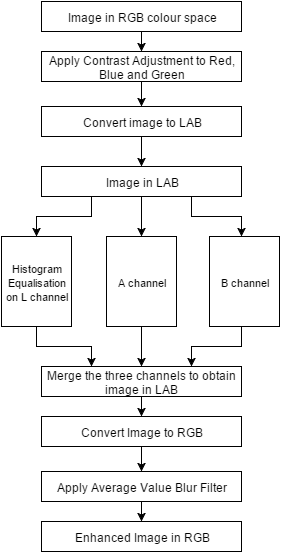
\includegraphics[width=0.42\textwidth]{figures/flowchart}
\caption{A flowchart of the proposed enhancement method. It shows the steps of that will be performed in the enhancement.}
\label{fig:flowchart}
\end{figure}

\section{Methodology}
\label{sec:methods}

% Blur Filter >
%  RGB TO LAB, 
% Histogram Equalisation, 
% Lab to RGB, 
% Contrast Adjustment
In this section the methods behind the Average Value Blur Filter, Colour Space Conversion, Histogram Equalisation, and Contrast Adjustment is described. A high-level overview of how the method works, a mathematical outline and pseudocode are also provided.
%In this section the methodology behind the mean matching approach to image enhancement is described.  As well as a high-level overview of how the method works, a mathematical outline and pseudocode are also provided.

\subsection{High-level Overview}
The idea behind the proposed automatic enhancement approach is to apply a Average Value Blur Filter for noise removal, then do a Histogram Equalisation on the Luminosity channel in LAB(CIELAB) to enhance the on the picture, then convert back to RGB and do a contrast adjustment. The enhancement will follow the flowchart on figure \ref{fig:flowchart}.

%TODO remove -> The basic idea behind the proposed automatic enhancement approach is to adjust the brightness of a given image such that its histogram is centred at the middle point of the intensity range.  For an 8-bit grayscale image, this middle value would correspond to $127$.  To achieve this mid-mean alignment, the intensity spectrum of the image is shifted such that the mean for each channel lies at $127$.  For a $24$-bit true colour image the method is applied in the same manner for each colour channel.  To find the adjustment amount for each colour channel, the offset between the actual mean, and the ``ideal'' mean (in this case $(K-1)/2$ or $127$) is computed.  This value is then added to each pixel to provide the brightness adjustment.

\begin{algorithm}[tp!]
\caption{Mid-Mean Alignment Algorithm}
\label{alg:mma}
\begin{algorithmic}[1]
\Function{MeanAligment} {$I$} \Comment{where $| I | = m \times n$}
	\State $I' = \mbox{zeros}(m, n, 3)$
	\State $\mu_{\mbox{\tiny{ideal}}} = [127, 127, 127]$
	\State $\mu_{\mbox{\tiny{actual}}} = [0, 0, 0]$
	\State 
	\For{\textbf{each} $p$ \textbf{in} $I$} 
		\State $\mu_{\mbox{\tiny{actual}}} = \mu_{\mbox{\tiny{actual}}} + p$
	\EndFor
	\State
	\State $\mu_{\mbox{\tiny{actual}}} = \mu_{\mbox{\tiny{actual}}} / (m \times n)$
	\State $s = \mu_{\mbox{\tiny{ideal}}} - \mu_{\mbox{\tiny{actual}}}$
	\State 
	\For{\textbf{each} $(p, p')$ \textbf{in} $(I, I')$} 
		\State $p' = \mbox{Clamp(}p + s$)
	\EndFor
	\State 
	\State
	\Return $I'$
\EndFunction
\end{algorithmic}
\end{algorithm}

\begin{figure}[b]
\centering
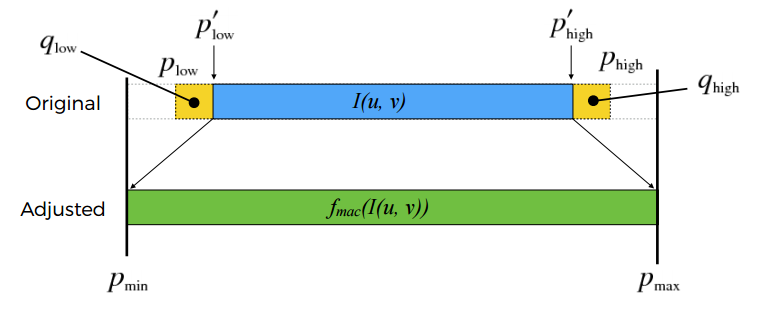
\includegraphics[width=0.42\textwidth]{figures/contrAdj.png}
\caption{An image showing how the range of values will be set when applying contrast adjustment to the picture.}
\label{fig:contrAdj}
\end{figure}

\begin{algorithm}[b!] %normal hist
	\caption{Normal Histogram}
	\label{alg:norm_hist}
	\begin{algorithmic}[1]
		\Function{NormalHistogram} {$I$} \Comment{where $| I | = m \times n$, \\ $K = 256$}
		\State $H = [0, K-1]$
		\State 
		\For{\textbf{each} $p$ \textbf{in} $I$} 
		\State $H(p) = H(p) + 1$
		\EndFor
		\State 
		\State
		\Return $H$
		\EndFunction
	\end{algorithmic}
\end{algorithm}
\begin{algorithm}[tp!]%cumulative hist
	\caption{Cumulative Histogram}
	\label{alg:cum_hist}
	\begin{algorithmic}[1]
		\Function{CumulativeHistogram} {$I$} \Comment{where $K = 256$}

		\State $H = $ NormalHistogram()
		\State $CH = [0, K-1]$
		\State
		\For{\textbf{each} $v$ \textbf{in} $H$} 
		\State $CH[v] = CH[v] + H[v]$
		\EndFor
		\State 
		\State
		\Return $I'$
		\EndFunction
	\end{algorithmic}
\end{algorithm}

\subsection{Detailed Description}

The proposed enhancement algorithm is a combination of filter and point-based histogram operations. To simplify the description of the operations, the algorithms assume that the picture is grayscale, however the final algorithm works on RGB images, by repeating the functions for each color channel. 
The first operation in the algorithm, the Average Value Blur is a filter, because it does not rely solely on a single pixel's value. The described filter operation acts on each channel in the same manner, using a filter operation function $f$, with width 3, meaning it takes the neighbouring pixels of the current pixel\cite{averageFilter}. That is: 
%TODO add pseudo code?
\begin{equation} %equation that shows filter calculation
	I'(u, v) = f(\frac{1}{9}\cdot\sum_{j=-1}^{1}\sum_{i=-1}^{1}I(u+i, v+j))
\end{equation}

The other two operations both rely on histograms to perform their operations. A histogram is a graphical representation of a distribution of numerical data\cite{histDesc}\cite{histDescWiki}. Figure \ref{fig:hist_comp} shows both a normal histogram and a cumulative histogram, both of which are used. The pseudocode for creating a normal histogram \ref{alg:norm_hist}, and the pseudocode for creating a cumulative histogram from the normal histogram \ref{alg:cum_hist} are included in the paper. The equation for deriving a cumulative histogram from a normal histogram can be simply written as: 
\begin{equation}%equation for cumulative histogram
\begin{aligned}
H(i) &=  \sum_{j = 0}^{i}h(j) 
& for(0 \leq i < K)
\end{aligned}
\end{equation}

\begin{figure}[h] % normal and cumulative histograms shown
	\centering
	\subfigure[original] {
		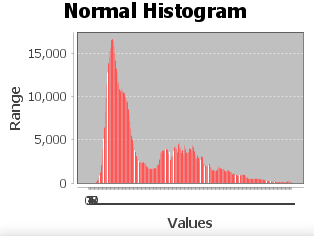
\includegraphics[width=0.2\textwidth]{figures/norm_hist.png}
	}
	\subfigure[modified] {
		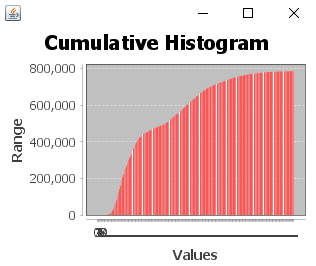
\includegraphics[width=0.2\textwidth]{figures/cum_hist.png}
	}
	\caption{Two images showing a normal histogram and a cumulative histogram of it.}
	\label{fig:hist_comp}
\end{figure}
\begin{figure}
	\centering
%	\includegraphics[width=0.2\textwidth]{figues/cum_hist_range.png}
\end{figure}
The second operation, the Contrast Adjustment, is performed on the image in RGB colour space, so no conversion is needed. Often the full range of values isn't used. Automatic contrast adjustment remaps the intensity values so that they occupy the full range of possible values\cite{automaticContrast}. We have to identify two quantiles at the low and high end of the intensity spectrum, and map the pixel values inside them to the extreme values, the other pixels are then linearly mapped to the interval [$p_{min}, p_{max}$] \ref{fig:contrAdj}. To calculate the two quantiles we set a range for ignored pixels $q$. Using that range we can calculate the quantiles using the cumulative histogram:
\begin{equation}
\begin{aligned}
&p'_{low} = \min\{i \| H(i) \geq m\cdot n \cdot q_{low}\}\\
&p'_{high} = \max\{i \| H(h) \leq m\cdot n \cdot q_{high}\}
\end{aligned}
\end{equation}
we get the ranges \includegraphics[width=0.2\textwidth]{figures/cum_hist_range.png}
%TODO finish writing the contrast adjustment, refer to lecture, https://blackboard.aber.ac.uk/bbcswebdav/pid-688647-dt-content-rid-1002902_1/courses/CS24110_AB0_2015-16/CS241_L09_LQ.pdf is the link for the slides, first do histogram and cumulative histogram, which can be re-used for LAB EQ later, then add equation for contrast adjustment

%other two operations, the Contrast Adjustment and the Luminosity equalisation, are both point-based histogram operations.
%The proposed mid-mean alignment algorithm is a point operation that acts on each colour channel in the same manner.  To simplify the description of the operation, the algorithm is described in terms of operating upon a single grayscale image.  However, it is worth noting that the final algorithm works on an RGB image and so the described approach is repeated for each colour channel.  The described point operation takes as input a grayscale image $I(u, v)$ of size $m \times n$ and produces an enhanced image $I'(u, v)$ using a point operation function $f$.  That is:

\noindent where $f$ is a homogeneous point operation and the geometry of $I'$ is exactly the same as $I$.

The point operation is sought such that the mean of the modified image matches some given mean (i.e. $(K-1)/2$).  This ``ideal'' mean is represented as $\mu$ and for an $8$-bit image, $\mu = 127$.  If, $\overline{I(u, v)}$ represents the mean of image $I$, then the point operation, $f$, is sought such that

\begin{equation}
	\overline{f(I(u, v))} = \mu
\end{equation}

\noindent that is, the mean of modified image equals $127$.

As shown in the sketch in Figure \ref{fig:sketch}, to perform this mean shift operation the mean of the image needs to be found and the difference between the actual mean and idea mean needs to be added to each pixel.  The actual mean, $\mu_{\mbox{\tiny{actual}}}$ is found via

\begin{equation}
	\mu_{\mbox{\tiny{actual}}} = \frac{1}{m \times n}\sum_{i=1}^{m \times n} p_{i}
\end{equation}

\noindent where is a single pixel, $p_{i} \in I(u, v)$.  The ideal mean for an $8$-bit image is given as $\mu_{\mbox{\tiny{ideal}}} = 127$ and so the final point operation is given as

\begin{equation}
	f(I(u, v)) = I(u, v) + (\mu_{\mbox{\tiny{ideal}}} - \mu_{\mbox{\tiny{actual}}})
\end{equation}

Therefore, for each pixel in each channel in the image, the shift amount between the actual mean and the ideal mean is added and so the mean of the output image will be aligned so that it corresponds to the mid-level intensity value.

\subsection{Implementation}

The description in the previous section is focussed on a single colour channel; however, since the algorithm needs to work on RGB images, the above method will need to be repeated for each colour channel.  To achieve this, the implementation will need to keep track of the actual mean values for the three colour channels separately and then ensure that the correct shift is applied to each colour channel.  As well as this, a clamping operation will need to be employed so that the modified intensities do not fall out of the displayable range of intensities.

The pseudocode algorithm is given in Algorithm \ref{alg:mma}.  The function takes as input an RGB $m \times n$ image $I$ and then starts by producing a blank output image of the same dimensions (line 2).  The ideal means are then given and lines 4-10 loop through the input image summing each pixel channel and then dividing by the total number of pixels to produce the actual mean (note, this divide is an element-wise divide so that each element in the actual vector is divided by $m \times n$).   Once the actual mean is calculated, the shift is found for each channel by subtracting the actual mean from the ideal mean (line 11).  Finally, the output image is filled by adding the shift amount to each pixel value found in the input image making sure that the pixels are clamped into the range $[0,255]$.  The function returns the modified image (line 17).

The implementation described in Algorithm 1 requires two loops through the image but using an efficient pixel accessing mechanism (i.e. Java's \texttt{WritableRaster} \cite{JavaWR}) then the run-time for this operation should be minimal.

\begin{figure*}[t]
	\centering
	\subfigure[Image 1 Original]{
		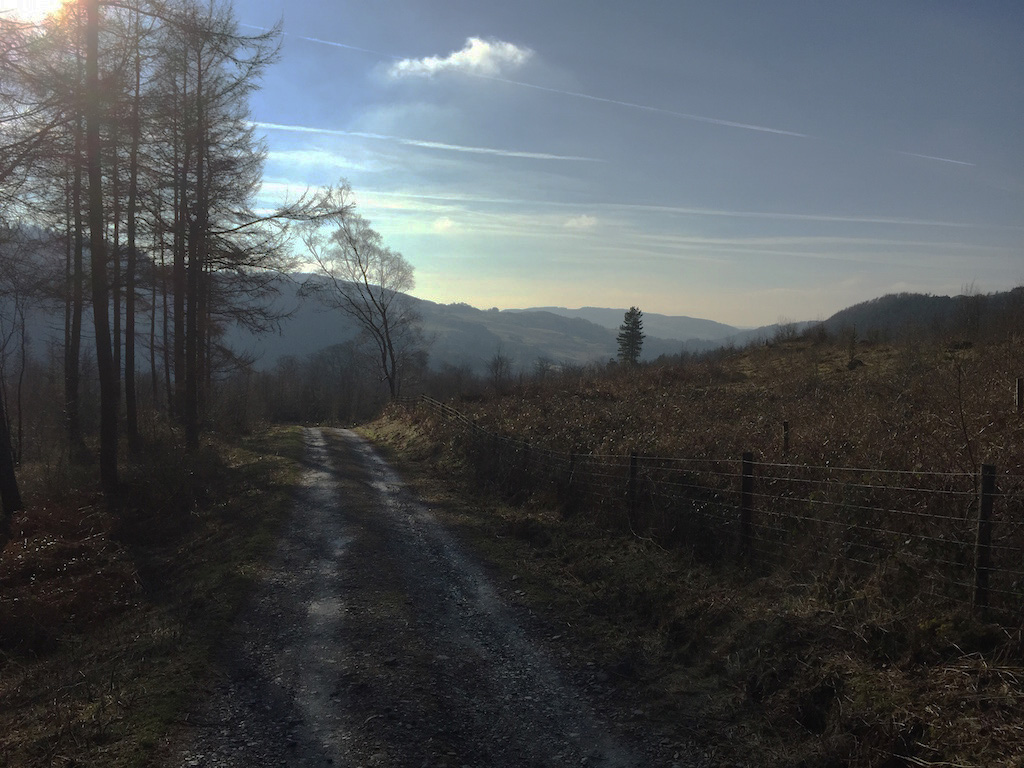
\includegraphics[width=0.225\textwidth]{figures//images//image_01.jpg}
	}
	\subfigure[Image 1 Modified]{
		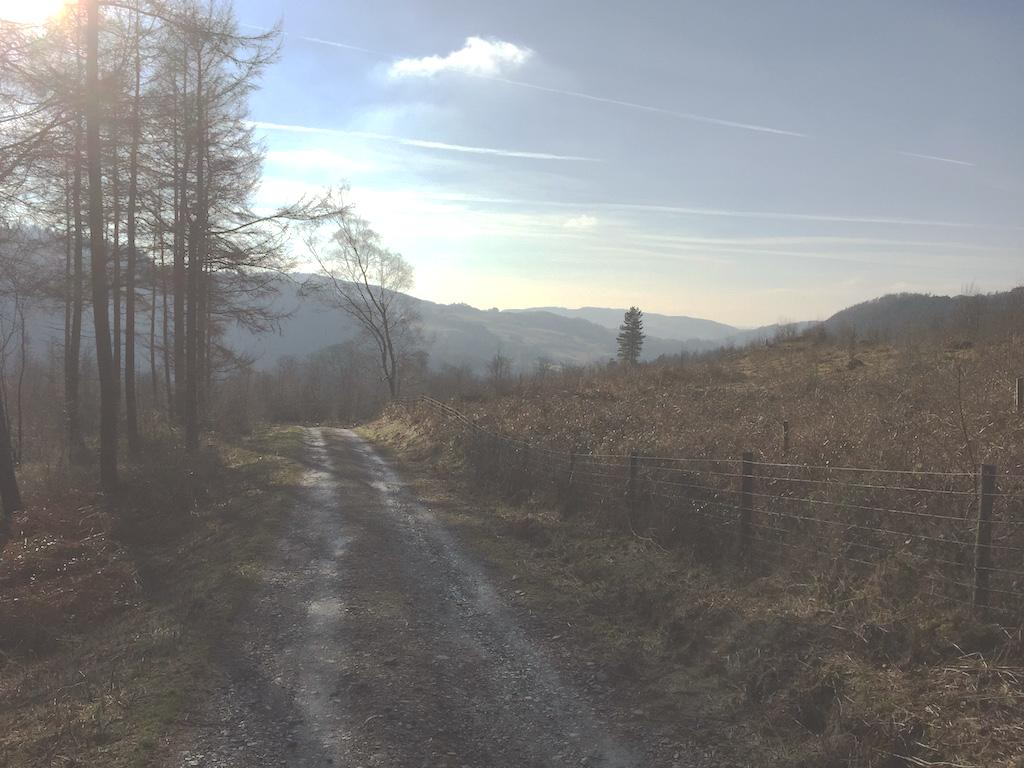
\includegraphics[width=0.225\textwidth]{figures//images//image_01_changed.jpg}
	} 
	\subfigure[Image 2 Original]{
		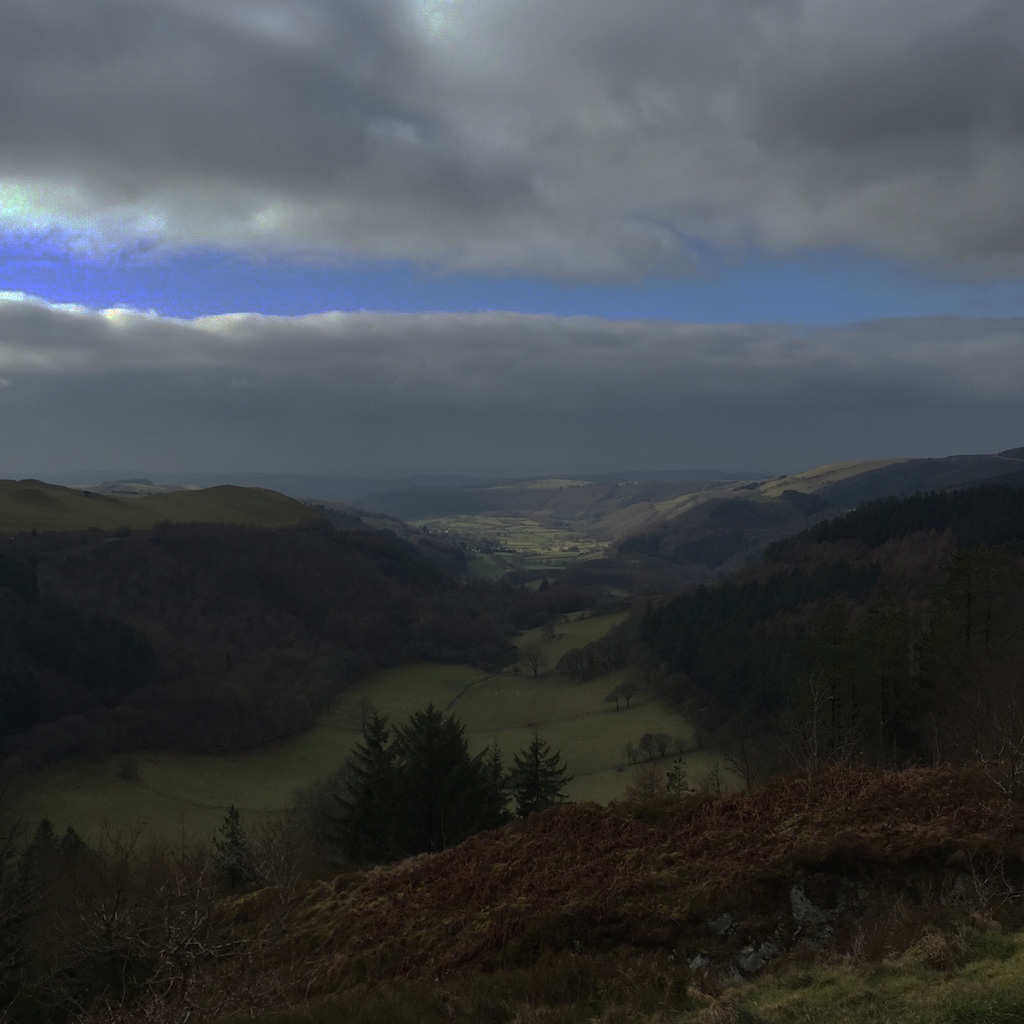
\includegraphics[width=0.225\textwidth]{figures//images//image_02.jpg}
	}
	\subfigure[Image 2 Modified]{
		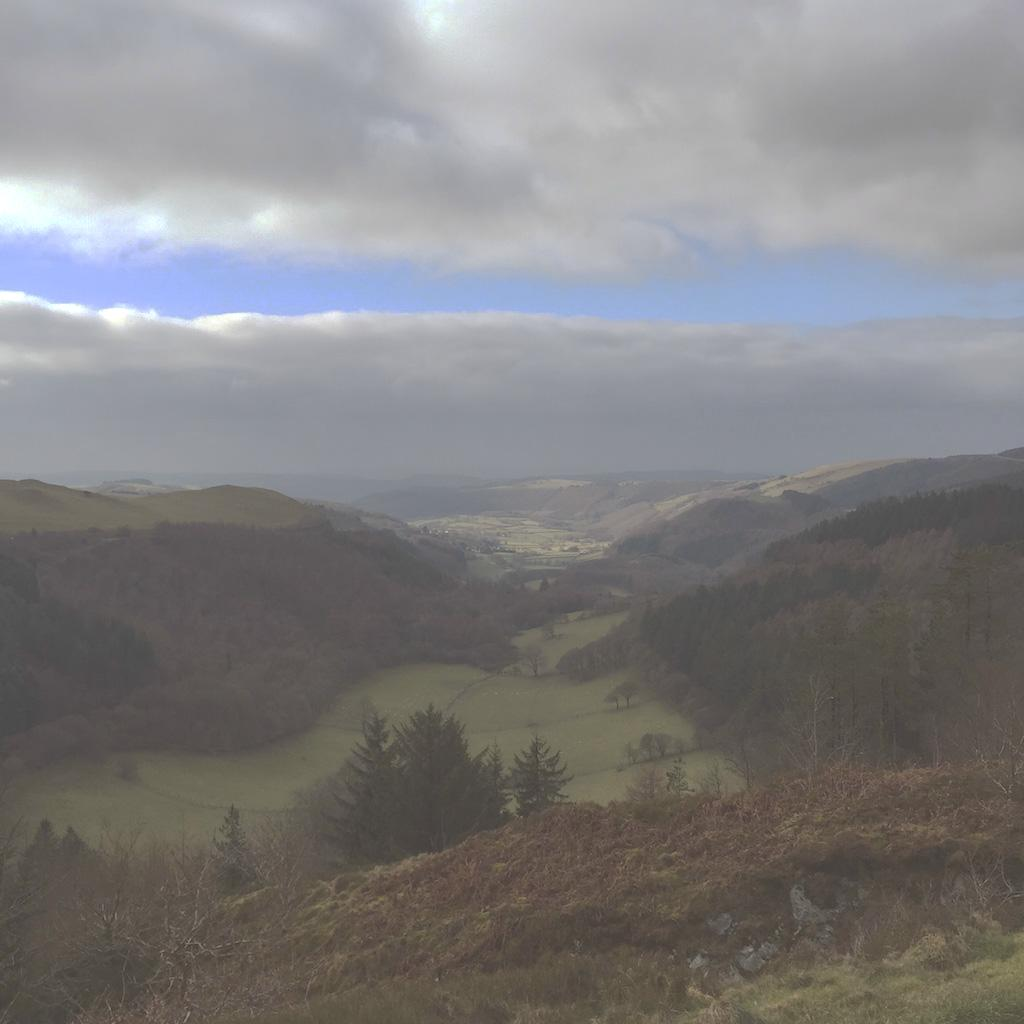
\includegraphics[width=0.225\textwidth]{figures//images//image_02_changed.jpg}
	} \\
	\subfigure[Image 3 Original]{
		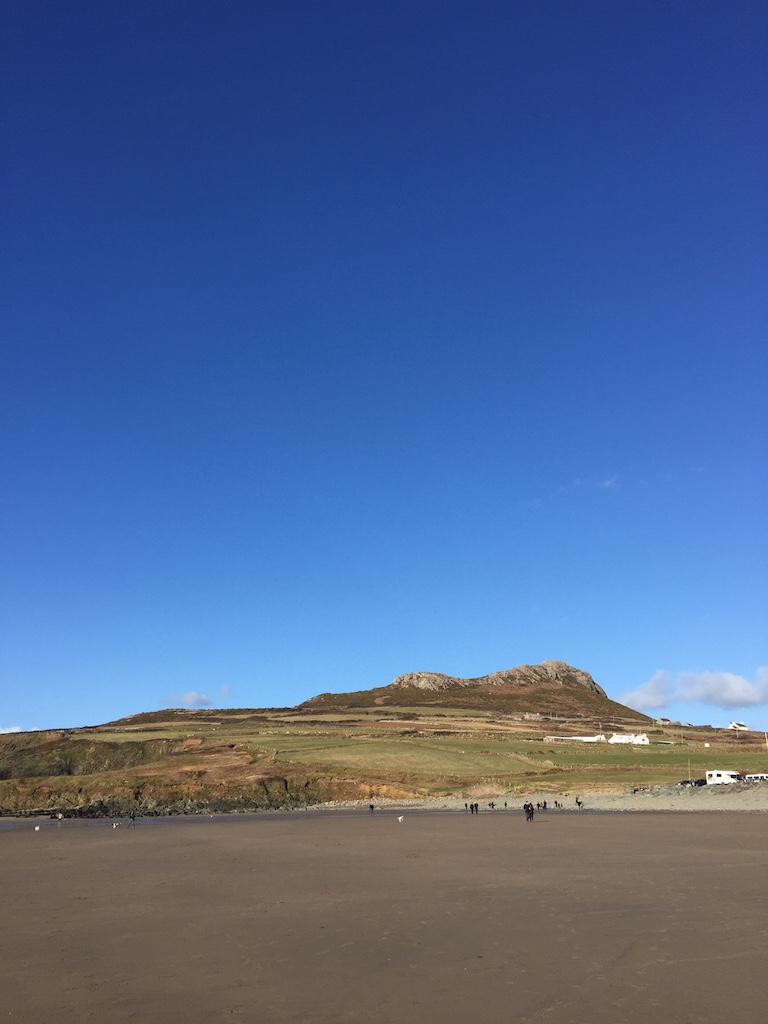
\includegraphics[width=0.225\textwidth]{figures//images//image_03.jpg}
	}
	\subfigure[Image 3 Modified]{
		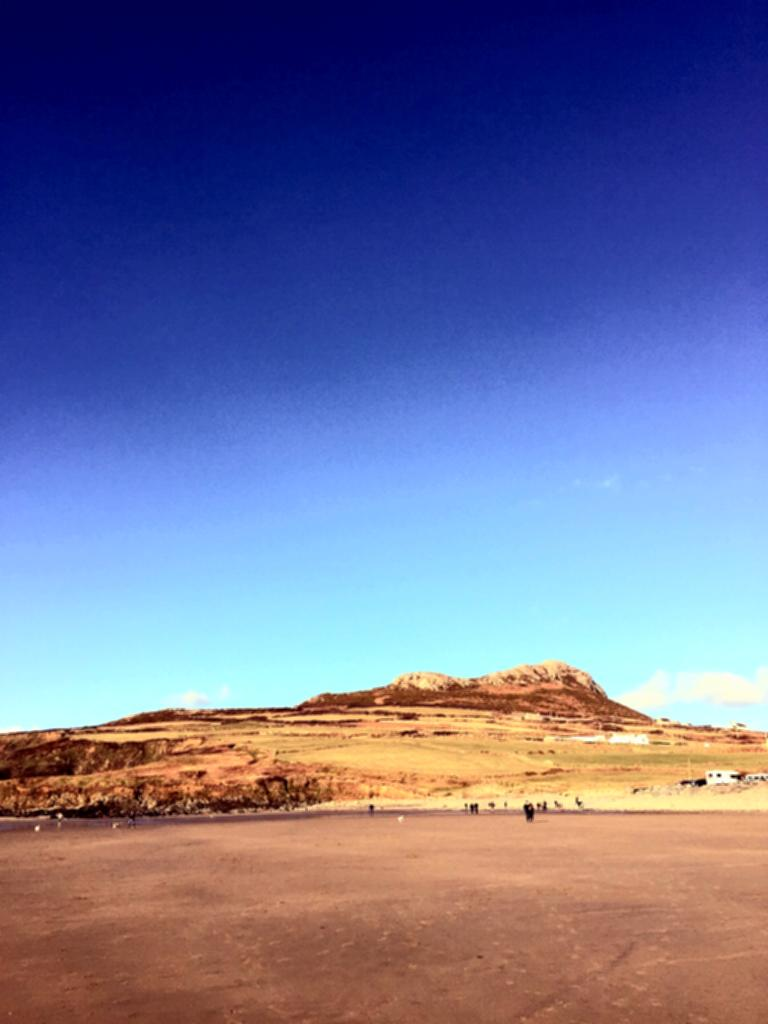
\includegraphics[width=0.225\textwidth]{figures//images//image_03_changed.jpg}
	} 
	\subfigure[Image 4 Original]{
		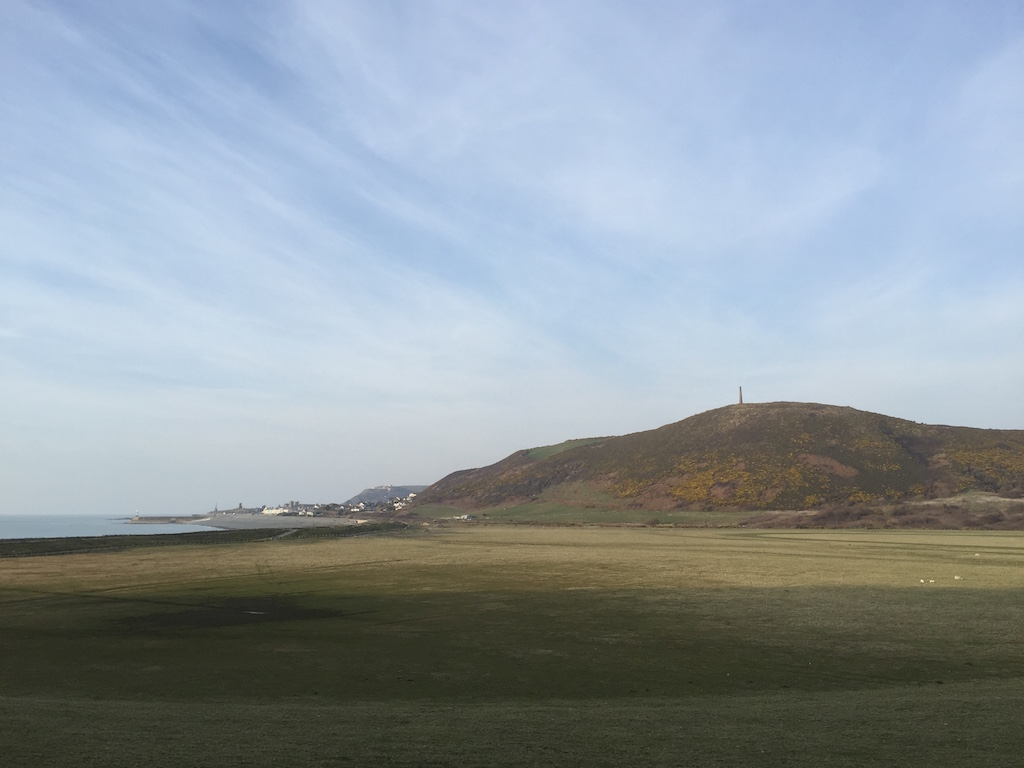
\includegraphics[width=0.225\textwidth]{figures//images//image_04.jpg}
	}
	\subfigure[Image 4 Modified]{
		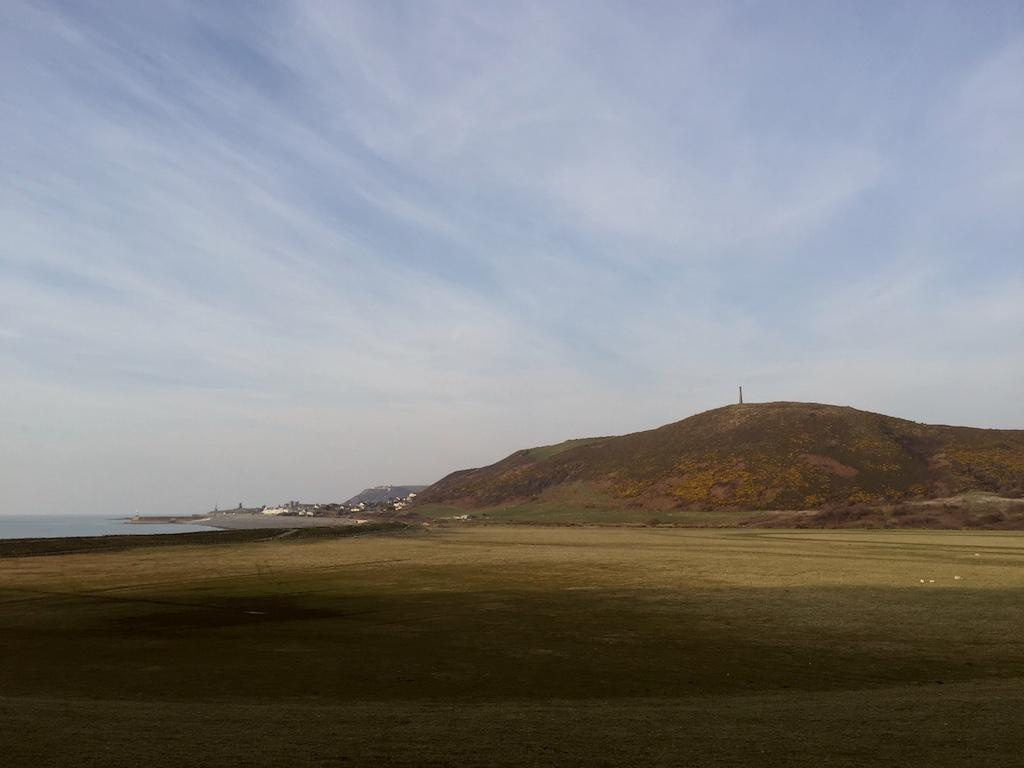
\includegraphics[width=0.225\textwidth]{figures//images//image_04_changed.jpg}
	} \\
	\subfigure[Image 5 Original]{
		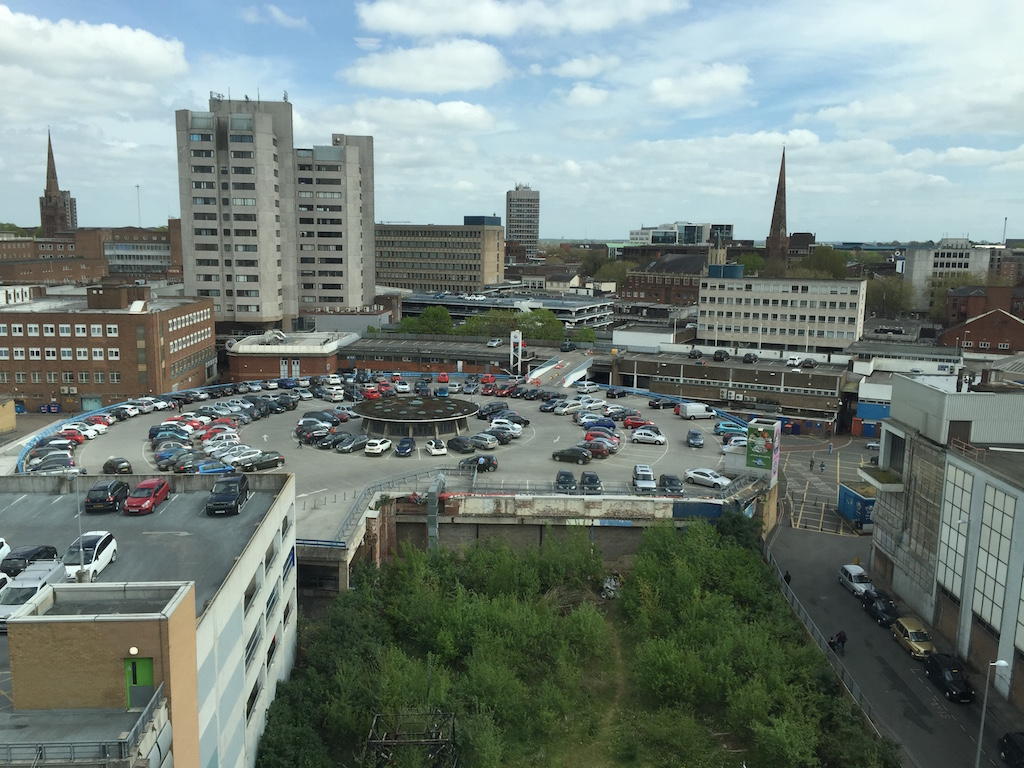
\includegraphics[width=0.225\textwidth]{figures//images//image_05.jpg}
	}
	\subfigure[Image 5 Modified]{
		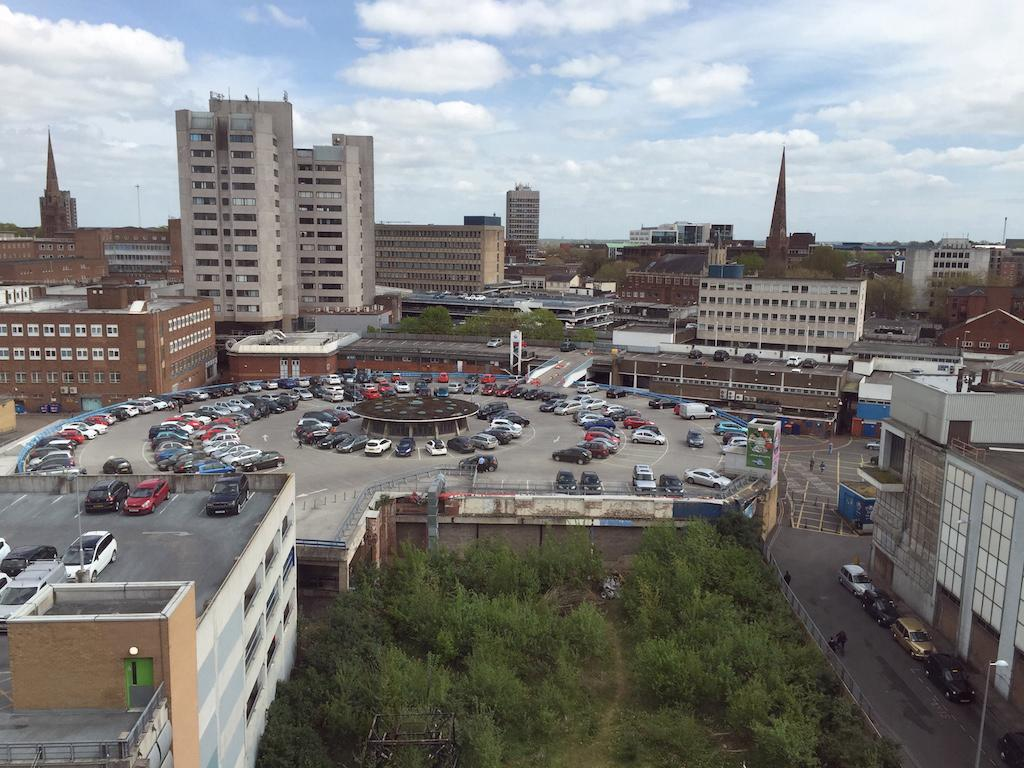
\includegraphics[width=0.225\textwidth]{figures//images//image_05_changed.jpg}
	} \\
\caption{Results of performing the mean alignment algorithm on each of the five test images.  For the first two images (a, c), the algorithm produces washed out results (b, d).  Performing the algorithm on Image 3 (e) causes a drastic change in colour (f), whereas the results for Image 4 (g) are far more natural (h).  The effect of the algorithm is least noticeable on Image 5 (i, j).}
\label{fig:results}
\end{figure*}

\begin{figure}[b]
	\centering
	\subfigure[original] {
		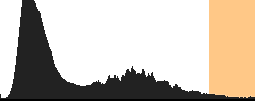
\includegraphics[width=0.2\textwidth]{figures//image01_hist.png}
	}
	\subfigure[modified] {
		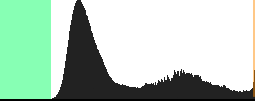
\includegraphics[width=0.2\textwidth]{figures//image_01_modified_hist.png}
	}
\caption{Average RGB histograms from image 1 (Figure \ref{fig:results} (a, b)).  The washed out effect seen in Figure \ref{fig:results} (b) occurs because all of the pixels highlighted in the orange region are mapped to maximum intensity.  Also note the range of unfilled intensities in the darker region of the modified image (green bar).}
\label{fig:image01_hists}
\end{figure}

\section{Results}
\label{sec:results}

The proposed method is tested on the provided four images.  The results of performing the mid-mean alignment algorithm on each of these images are shown in Figure \ref{fig:results}.

In all of the images the algorithm causes a change in the modified image, with the least significant change being seen in Image 5 (Figure \ref{fig:results} (i, j)).  Although the change is least significant for Image 5, it is only Image 5 and Image 4 that have natural looking results; all the other images, when modified, appear either washed out or with large colour changes.  

The modified versions of Images 1 and 2 both appear washed out.  This can be explained when the histograms are examined.  Figure \ref{fig:image01_hists} shows the histogram before and after processing for Image 1.  The washed out effect occurs because all of the pixels within the shaded orange region in the original image are mapped to maximum intensity in the final image.  As well as this, the full range of intensities are not used in the final image so that image will appear to have low contrast.  This identifies an important property of the proposed algorithm, although it only performs a brightness adjustment, the algorithm can also modify contrast.  This is due to the fact that large shifts in intensity (such as those seen in Figure \ref{fig:image01_hists}) will cause a large block of pixels to be mapped to the extreme values.  The remaining pixels will be shifted as normal but the range of intensities used will be decreased thus leading to a decrease in contrast.

\begin{table}[t]
\centering
\normalsize{
\begin{tabular}{ l c c c c}

	\toprule
  Image	&	$s_{\mbox{\tiny{red}}}$	& $s_{\mbox{\tiny{green}}}$	& $s_{\mbox{\tiny{blue}}}$  & $\delta s$\\
  \midrule
  Image 1	&      $+53$				& $+49$					& $+46$ 				& $7$\\
  Image 2	&      $+63$				& $+58$					& $+55$ 				& $8$ \\	
  Image 3	&      $+49$				& $+25$					& $-21$ 				& $70$\\
  Image 4	&      $-14$				& $-24$					& $-31$ 				& $17$ \\
  Image 5	&      $+12$				& $-1$					& $+4$ 				& $13$\\
  \bottomrule
  \vspace{5pt}
\end{tabular}
}
\caption{The different shifts for each colour channel for each image.  The larger the shift the greater the effect; the larger the difference in shifts between each colour channel the greater the colour changes will be.}
\label{tbl:shifts}
\end{table}

The colour change that is seen in Image 3 (Figure \ref{fig:results} (e, f)) occurs because the shifting operation has a larger effect on a single colour channel.  The proposed method shifts each colour channel by a separate amount, so if, say, the green channel has a larger shift than the red and blue channels then the modified image will display a marked change in the green component (either more green or less green).  This effect can be further understood by examining the shift amounts for each colour channel for each image.   Table \ref{tbl:shifts} shows the shift amounts for each colour channel for each image as well as the size of the shift (measured as the range of the shift values for that image).  As can be seen, the cases when there is a large $\delta s$ correspond to cases when there is a significant change in colour.   Similarly, cases where there is a large shift even though there is a small $\delta s$, correspond to cases where there are contrast changes.



% [53, 49, 46]
%[63, 58, 55]
%[49, 25, -21]
%[-14, -24, -31]
%[12, -1, 4]

\section{Discussion \& Conclusions}
\label{sec:discussion}

The results show that the proposed method works best when there is a small shift observed for each colour channel and the difference in shifts between each colour channel is minimal.  If the shift amount is large, then it is likely that the image will appear washed out and the image's contrast will change.  Also, if the shift amount is very different for each colour channel, then the modified image will contain a very different colour distribution than the original image.   

Therefore, a few key properties of the algorithm can be noted:

\begin{enumerate}
\item The algorithm works best when the shift factor ($\mu_{\mbox{\tiny{ideal}}} - \mu_{\mbox{\tiny{actual}}}$ in Equation 4) is small.  If the shift factor is large then it is likely that a contrast change will be observed.
\item If the distribution of intensities across the different colour channels are very different, then the algorithm will produce an image with colour changes.
\item The algorithm will work best when the distribution of intensities are distributed in an approximately Gaussian distribution. 
\end{enumerate}

With these properties in mind it is possible to outline some possible areas for future improvement.  Firstly, it would be beneficial to incorporate some kind of contrast adjustment \emph{after} the brightness shift has occurred.  This would enable the contrast changes seen in Figure \ref{fig:results} (b) and (d) to be alleviated.  However, it is worth noting that performing a post-processing contrast adjustment would mean that the mean of the target image is no longer aligned to the middle value.

Secondly, the colour problem could be alleviated by performing the shifting operation in a different colour space.  For example, using the HSV colour space would allow for the brightness information to be treated separately from the colour information.  This would reduce the problem to be a single dimensional shift and so the changes in colour that can be seen in the current algorithm could be removed.

Thirdly, the shifting information shown in Table \ref{tbl:shifts} could be used to quantify the effect of the algorithm and so could be used to help guide further processing.  For example, if a low $\delta s$ value is observed then it is likely that no further processing is needed; however, if a high $\delta s$ value is observed then it is likely that the colour information has changed and so further processing, or even different processing, may be required.

In conclusion, this paper has presented a method for automatic image enhancement based on shifting the pixel intensities for each colour channel so that they are mean-aligned to the middle intensity value.  This mid-mean alignment algorithm is intuitive and easy to implement.  In some cases the method is able to improve the quality of the image without any contrast or colour artefacts.  However, in other cases the method, although simple, changes both the colour and the contrast of the image.  This may not be a desirable feature and so further processing, or performing this algorithm in a different colour space, may help overcome these issues.  It is expected that the proposed method could form the basis for a more advanced processing pipeline, and the shift information gained as a result of performing this mid-mean alignment algorithm could give important information to help guide the user in further enhancement processing.

% can use a bibliography generated by BibTeX as a .bbl file
% BibTeX documentation can be easily obtained at:
% http://www.ctan.org/tex-archive/biblio/bibtex/contrib/doc/
% The IEEEtran BibTeX style support page is at:
% http://www.michaelshell.org/tex/ieeetran/bibtex/
\bibliographystyle{IEEEtran}
% argument is your BibTeX string definitions and bibliography database(s)
\bibliography{biblio}


% if you will not have a photo at all:
% that's all folks
\end{document}


